%%Copyright 2021. Any replication of this document is permissible. The primary package of this document is from cjquines%%

%%PRIMARY PREAMBLE%%
\documentclass[12pt,paper=letter]{scrartcl}
\usepackage[ boxthm, parskip]{cjquines}
\usepackage{CJKutf8}


%%ADDITIONAL PACKAGES%%

\tikzset{every picture/.style={line width=0.75pt}} %set default line width to 0.75pt 
\newcommand{\ans}[1]{{\sffamily \bfseries Answer.}\;\(\boxed{\text{#1}}\).}
\newcommand{\ansb}[2]{{\sffamily \bfseries Answer.}\;\(\boxed{\text{(#1) #2}}\).}
\newcommand{\sol}{{\sffamily \bfseries Solution.}\;}
\newcommand{\soln}[1]{{\sffamily \bfseries Solution #1.}\;}
\newcommand{\back}[1]{{\sffamily \bfseries Background.}\;}
\newenvironment{rem}%
{\noindent \ignorespaces \small \sffamily \sansmath {\bfseries Remark.}}%
{\ignorespacesafterend}

\newcommand{\joshbluebf}[1]{{\bfseries \sffamily \color{DarkMidnightBlue} #1}}
\newcommand{\joshbf}[1]{{\bfseries \sffamily \color{black} #1}}



%%FONT FAMILY%%
%\renewcommand{\familydefault}{\sfdefault}%


\begin{document}


\title{Week 6 Some Random Problems}
\author{\joshbluebf{Problems of the Week — Season 2}}
\date{February 4, 2022}

\maketitle
\setlength{\unitlength}{1in}
\begin{picture}(2,0)
  \put(1.20,1.45){\hbox{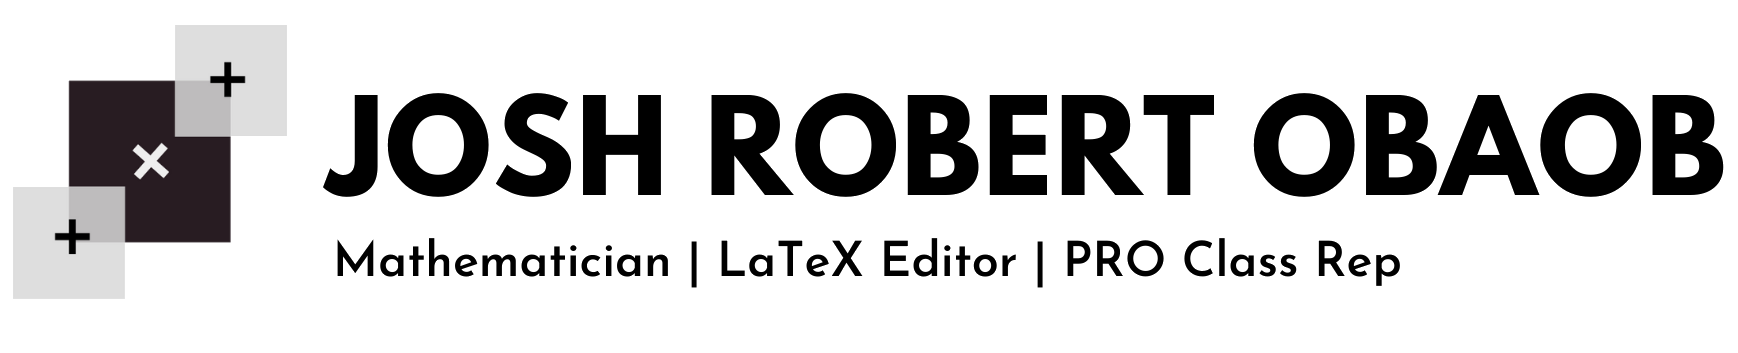
\includegraphics[width=4.2in]{logo2.png}}}
\end{picture}
\vspace{-2em}


\begin{abstract}
Hi! This is the \joshbf{sixth episode/article} of my mathematical series. In this article, this contains some random problems from Art of Problem Solving website. Enjoy!
\end{abstract}

\vspace{-2em}

\section*{Problems}


\begin{problem}
 Tej is typing a string of $L$s and $O$s that consists of exactly $7$ $L$s and $4$ $O$s. How many different strings can he type that do not contain the substring ‘$LOL$’ anywhere? A substring is a sequence of consecutive letters contained within the original string.
\end{problem}

\begin{problem}
Given three distinct unit circles (i.e. circles of radius $1$), each of which is tangent to the other two, find the radius of the circle which is tangent to all three circles and contains them.

\begin{center}
    


\tikzset{every picture/.style={line width=0.75pt}} %set default line width to 0.75pt        

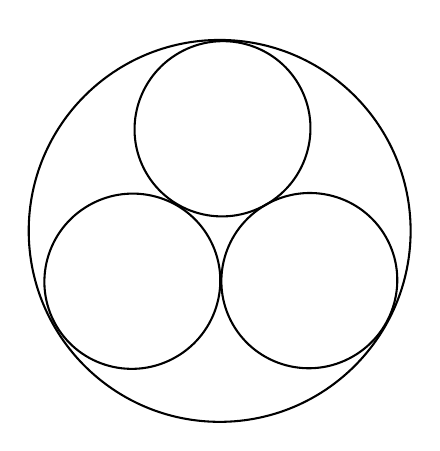
\begin{tikzpicture}[x=0.75pt,y=0.75pt,yscale=-1,xscale=1]
%uncomment if require: \path (0,300); %set diagram left start at 0, and has height of 300

%Shape: Circle [id:dp5294208793352049] 
\draw   (204.78,140.94) .. controls (204.78,90.13) and (245.97,48.94) .. (296.78,48.94) .. controls (347.59,48.94) and (388.78,90.13) .. (388.78,140.94) .. controls (388.78,191.75) and (347.59,232.94) .. (296.78,232.94) .. controls (245.97,232.94) and (204.78,191.75) .. (204.78,140.94) -- cycle ;
%Shape: Ellipse [id:dp04719336738451996] 
\draw   (277.23,55.16) .. controls (297.58,43.53) and (323.45,50.47) .. (335,70.67) .. controls (346.55,90.87) and (339.41,116.68) .. (319.06,128.32) .. controls (298.71,139.96) and (272.84,133.02) .. (261.29,112.81) .. controls (249.74,92.61) and (256.88,66.8) .. (277.23,55.16) -- cycle ;
%Shape: Ellipse [id:dp15175862857444034] 
\draw   (319.06,128.32) .. controls (339.41,116.68) and (365.28,123.63) .. (376.83,143.83) .. controls (388.38,164.03) and (381.24,189.84) .. (360.89,201.48) .. controls (340.54,213.12) and (314.67,206.17) .. (303.12,185.97) .. controls (291.57,165.77) and (298.71,139.96) .. (319.06,128.32) -- cycle ;
%Shape: Ellipse [id:dp27659456991302744] 
\draw   (233.78,128.61) .. controls (254.14,116.97) and (280,123.92) .. (291.55,144.12) .. controls (303.1,164.32) and (295.97,190.13) .. (275.61,201.77) .. controls (255.26,213.41) and (229.4,206.46) .. (217.85,186.26) .. controls (206.3,166.06) and (213.43,140.25) .. (233.78,128.61) -- cycle ;




\end{tikzpicture}
\end{center}
\end{problem}

\begin{problem}
 Find all real numbers $x$ which satisfy $\sin x + \cos x =\sqrt{\dfrac{2 + \sqrt3}{2}}$, with $0 < x < \dfrac{\pi}{2}$
\end{problem}

\begin{problem}
There exists a $\Delta ABC$ such that $\overline{AB}=5, \overline{BC} =10$ and there exists a point $D$ such that $\overline{BD}$ is an angle bisector of $\angle ABC = 120^{\circ}$. Find the length of $\overline{BD.}$
\end{problem}

\begin{problem}[IMO Shortlist, 2004]
Find all functions $f:\mathbb{R} \to \mathbb{R}$ satisfying the equation\[
	f(x^2+y^2+2f(xy)) = (f(x+y))^2.
\]for all $x,y \in \mathbb{R}$.
\end{problem}



\newpage

\section*{Solutions}

\vspace{2mm}

\begin{probboxed}
Tej is typing a string of $L$s and $O$s that consists of exactly $7$ $L$s and $4$ $O$s. How many different strings can he type that do not contain the substring ‘$LOL$’ anywhere? A substring is a sequence of consecutive letters contained within the original string.
\end{probboxed}

\ans{78}

\sol

For this problem, we are going to invoke the concept of complementary counting, which states that:

$$P(A \cup B) - P(B) = P(A)$$

where $B$ is the complimentary set of $A$ such that there are no elements of $A$ can be found in $B$. Using the concept, we will treat $P(B)$ as the number of ways to have a string with $LOL$ in it. Counting the total ways to arrange the string, we have $\dfrac{11!}{7!4!} = 330$ ways to do this. Next, count the number of ways that we can form a string with $LOL$ sub-string, and we have $\dfrac{9!}{5!3!} \times \dfrac{1}{2!1!} = \dfrac{9!}{5!3!2!} = 252$ ways to do this. 

\vspace{2mm}

Invoking the complementary counting, we have $330-252$ = \fbox{78 ways}. and this is our final answer.

\begin{probboxed}
Given three distinct unit circles (i.e. circles of radius $1$), each of which is tangent to the other two, find the radius of the circle which is tangent to all three circles and contains them.

\begin{center}
    


\tikzset{every picture/.style={line width=0.75pt}} %set default line width to 0.75pt        

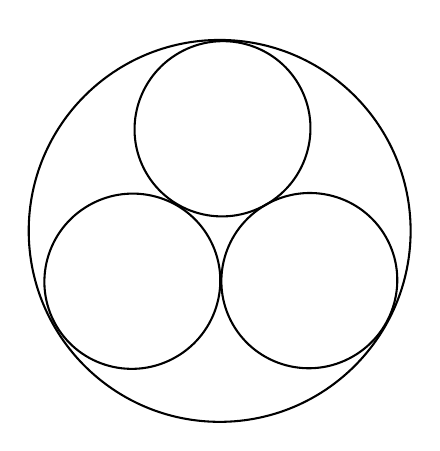
\begin{tikzpicture}[x=0.75pt,y=0.75pt,yscale=-1,xscale=1]
%uncomment if require: \path (0,300); %set diagram left start at 0, and has height of 300

%Shape: Circle [id:dp5294208793352049] 
\draw   (204.78,140.94) .. controls (204.78,90.13) and (245.97,48.94) .. (296.78,48.94) .. controls (347.59,48.94) and (388.78,90.13) .. (388.78,140.94) .. controls (388.78,191.75) and (347.59,232.94) .. (296.78,232.94) .. controls (245.97,232.94) and (204.78,191.75) .. (204.78,140.94) -- cycle ;
%Shape: Ellipse [id:dp04719336738451996] 
\draw   (277.23,55.16) .. controls (297.58,43.53) and (323.45,50.47) .. (335,70.67) .. controls (346.55,90.87) and (339.41,116.68) .. (319.06,128.32) .. controls (298.71,139.96) and (272.84,133.02) .. (261.29,112.81) .. controls (249.74,92.61) and (256.88,66.8) .. (277.23,55.16) -- cycle ;
%Shape: Ellipse [id:dp15175862857444034] 
\draw   (319.06,128.32) .. controls (339.41,116.68) and (365.28,123.63) .. (376.83,143.83) .. controls (388.38,164.03) and (381.24,189.84) .. (360.89,201.48) .. controls (340.54,213.12) and (314.67,206.17) .. (303.12,185.97) .. controls (291.57,165.77) and (298.71,139.96) .. (319.06,128.32) -- cycle ;
%Shape: Ellipse [id:dp27659456991302744] 
\draw   (233.78,128.61) .. controls (254.14,116.97) and (280,123.92) .. (291.55,144.12) .. controls (303.1,164.32) and (295.97,190.13) .. (275.61,201.77) .. controls (255.26,213.41) and (229.4,206.46) .. (217.85,186.26) .. controls (206.3,166.06) and (213.43,140.25) .. (233.78,128.61) -- cycle ;




\end{tikzpicture}
\end{center}
\end{probboxed}


\newpage

\ans{$\sqrt{3} + \dfrac{1}{2}$}

\sol

\begin{center}



\tikzset{every picture/.style={line width=0.75pt}} %set default line width to 0.75pt        

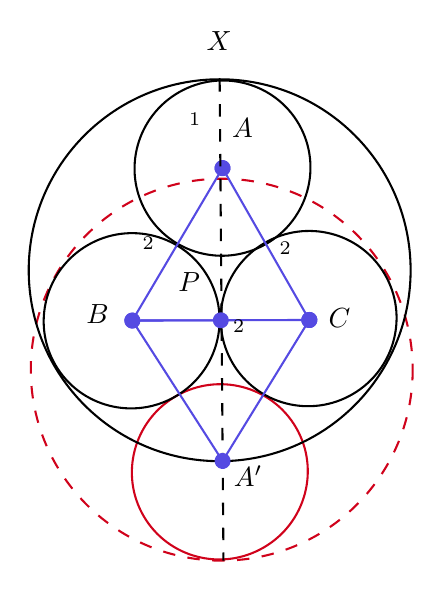
\begin{tikzpicture}[x=0.75pt,y=0.75pt,yscale=-1,xscale=1]
%uncomment if require: \path (0,614); %set diagram left start at 0, and has height of 614

%Shape: Circle [id:dp023383431999783877] 
\draw  [color={rgb, 255:red, 208; green, 2; blue, 27 }  ,draw opacity=1 ][dash pattern={on 4.5pt off 4.5pt}] (318.47,441.52) .. controls (318.94,492.33) and (278.12,533.89) .. (227.31,534.35) .. controls (176.5,534.81) and (134.94,494) .. (134.48,443.19) .. controls (134.02,392.38) and (174.83,350.82) .. (225.64,350.36) .. controls (276.45,349.9) and (318.01,390.71) .. (318.47,441.52) -- cycle ;
%Shape: Ellipse [id:dp6125140008012029] 
\draw  [color={rgb, 255:red, 208; green, 2; blue, 27 }  ,draw opacity=1 ] (246.8,527.96) .. controls (226.56,539.78) and (200.63,533.07) .. (188.9,512.97) .. controls (177.16,492.88) and (184.06,467) .. (204.31,455.18) .. controls (224.56,443.36) and (250.48,450.07) .. (262.22,470.16) .. controls (273.95,490.26) and (267.05,516.13) .. (246.8,527.96) -- cycle ;
%Shape: Ellipse [id:dp417107218858334] 
\draw   (204.31,455.18) .. controls (184.06,467) and (158.14,460.29) .. (146.41,440.2) .. controls (134.67,420.1) and (141.57,394.23) .. (161.82,382.4) .. controls (182.06,370.58) and (207.99,377.29) .. (219.72,397.39) .. controls (231.46,417.48) and (224.56,443.36) .. (204.31,455.18) -- cycle ;
%Shape: Ellipse [id:dp6585027419967555] 
\draw   (289.58,454.12) .. controls (269.34,465.94) and (243.41,459.23) .. (231.68,439.13) .. controls (219.94,419.04) and (226.84,393.16) .. (247.09,381.34) .. controls (267.34,369.52) and (293.26,376.23) .. (304.99,396.32) .. controls (316.73,416.42) and (309.83,442.29) .. (289.58,454.12) -- cycle ;
%Shape: Circle [id:dp37634332573409135] 
\draw   (133.48,394.44) .. controls (133.48,343.63) and (174.67,302.44) .. (225.48,302.44) .. controls (276.29,302.44) and (317.48,343.63) .. (317.48,394.44) .. controls (317.48,445.25) and (276.29,486.44) .. (225.48,486.44) .. controls (174.67,486.44) and (133.48,445.25) .. (133.48,394.44) -- cycle ;
%Shape: Ellipse [id:dp43980857374211935] 
\draw   (205.93,308.66) .. controls (226.28,297.03) and (252.15,303.97) .. (263.7,324.17) .. controls (275.25,344.37) and (268.11,370.18) .. (247.76,381.82) .. controls (227.41,393.46) and (201.54,386.52) .. (189.99,366.31) .. controls (178.44,346.11) and (185.58,320.3) .. (205.93,308.66) -- cycle ;
%Straight Lines [id:da5670427688873849] 
\draw [color={rgb, 255:red, 85; green, 74; blue, 226 }  ,draw opacity=1 ]   (226.85,345.24) -- (183.4,418.69) ;
\draw [shift={(183.4,418.69)}, rotate = 120.61] [color={rgb, 255:red, 85; green, 74; blue, 226 }  ,draw opacity=1 ][fill={rgb, 255:red, 85; green, 74; blue, 226 }  ,fill opacity=1 ][line width=0.75]      (0, 0) circle [x radius= 3.35, y radius= 3.35]   ;
\draw [shift={(226.85,345.24)}, rotate = 120.61] [color={rgb, 255:red, 85; green, 74; blue, 226 }  ,draw opacity=1 ][fill={rgb, 255:red, 85; green, 74; blue, 226 }  ,fill opacity=1 ][line width=0.75]      (0, 0) circle [x radius= 3.35, y radius= 3.35]   ;
%Straight Lines [id:da02689944550443535] 
\draw [color={rgb, 255:red, 85; green, 74; blue, 226 }  ,draw opacity=1 ]   (226.85,345.24) -- (268.68,418.4) ;
\draw [shift={(268.68,418.4)}, rotate = 60.24] [color={rgb, 255:red, 85; green, 74; blue, 226 }  ,draw opacity=1 ][fill={rgb, 255:red, 85; green, 74; blue, 226 }  ,fill opacity=1 ][line width=0.75]      (0, 0) circle [x radius= 3.35, y radius= 3.35]   ;
\draw [shift={(226.85,345.24)}, rotate = 60.24] [color={rgb, 255:red, 85; green, 74; blue, 226 }  ,draw opacity=1 ][fill={rgb, 255:red, 85; green, 74; blue, 226 }  ,fill opacity=1 ][line width=0.75]      (0, 0) circle [x radius= 3.35, y radius= 3.35]   ;
%Straight Lines [id:da19907923286841633] 
\draw [color={rgb, 255:red, 85; green, 74; blue, 226 }  ,draw opacity=1 ]   (268.68,418.4) -- (183.4,418.69) ;
\draw [shift={(183.4,418.69)}, rotate = 179.81] [color={rgb, 255:red, 85; green, 74; blue, 226 }  ,draw opacity=1 ][fill={rgb, 255:red, 85; green, 74; blue, 226 }  ,fill opacity=1 ][line width=0.75]      (0, 0) circle [x radius= 3.35, y radius= 3.35]   ;
\draw [shift={(268.68,418.4)}, rotate = 179.81] [color={rgb, 255:red, 85; green, 74; blue, 226 }  ,draw opacity=1 ][fill={rgb, 255:red, 85; green, 74; blue, 226 }  ,fill opacity=1 ][line width=0.75]      (0, 0) circle [x radius= 3.35, y radius= 3.35]   ;
%Straight Lines [id:da11982252202972754] 
\draw [color={rgb, 255:red, 0; green, 0; blue, 0 }  ,draw opacity=1 ] [dash pattern={on 4.5pt off 4.5pt}]  (225.48,302.44) -- (227.31,534.35) ;
%Straight Lines [id:da35232835561383413] 
\draw [color={rgb, 255:red, 85; green, 74; blue, 226 }  ,draw opacity=1 ]   (183.4,418.69) -- (226.89,486.33) ;
%Straight Lines [id:da6984444811603441] 
\draw [color={rgb, 255:red, 85; green, 74; blue, 226 }  ,draw opacity=1 ]   (268.68,418.4) -- (226.89,486.33) ;
\draw [shift={(226.89,486.33)}, rotate = 121.6] [color={rgb, 255:red, 85; green, 74; blue, 226 }  ,draw opacity=1 ][fill={rgb, 255:red, 85; green, 74; blue, 226 }  ,fill opacity=1 ][line width=0.75]      (0, 0) circle [x radius= 3.35, y radius= 3.35]   ;
\draw [shift={(268.68,418.4)}, rotate = 121.6] [color={rgb, 255:red, 85; green, 74; blue, 226 }  ,draw opacity=1 ][fill={rgb, 255:red, 85; green, 74; blue, 226 }  ,fill opacity=1 ][line width=0.75]      (0, 0) circle [x radius= 3.35, y radius= 3.35]   ;
%Straight Lines [id:da365365470511408] 
\draw [color={rgb, 255:red, 85; green, 74; blue, 226 }  ,draw opacity=1 ]   (226.04,418.55) -- (183.4,418.69) ;
\draw [shift={(226.04,418.55)}, rotate = 179.81] [color={rgb, 255:red, 85; green, 74; blue, 226 }  ,draw opacity=1 ][fill={rgb, 255:red, 85; green, 74; blue, 226 }  ,fill opacity=1 ][line width=0.75]      (0, 0) circle [x radius= 3.35, y radius= 3.35]   ;


% Text Node
\draw (204.12,393.9) node [anchor=north west][inner sep=0.75pt]    {$P$};
% Text Node
\draw (230.52,416.9) node [anchor=north west][inner sep=0.75pt]  [font=\scriptsize]  {$2$};
% Text Node
\draw (252.92,379.3) node [anchor=north west][inner sep=0.75pt]  [font=\scriptsize]  {$2$};
% Text Node
\draw (186.92,376.9) node [anchor=north west][inner sep=0.75pt]  [font=\scriptsize]  {$2$};
% Text Node
\draw (209.32,317.3) node [anchor=north west][inner sep=0.75pt]  [font=\scriptsize]  {$1$};
% Text Node
\draw (230.82,486.98) node [anchor=north west][inner sep=0.75pt]    {$A'$};
% Text Node
\draw (217.72,278.08) node [anchor=north west][inner sep=0.75pt]    {$X$};
% Text Node
\draw (276.52,411.28) node [anchor=north west][inner sep=0.75pt]    {$C$};
% Text Node
\draw (159.72,409.68) node [anchor=north west][inner sep=0.75pt]    {$B$};
% Text Node
\draw (230.02,320.08) node [anchor=north west][inner sep=0.75pt]    {$A$};


\end{tikzpicture}
\end{center}

Let be the bigger circle be $\lambda$, and let $A,B,C$ be the centers of the unit circles being inscribed in circle $\lambda$. For the sake of clarity, let us \textit{complete the figure} based on the given details in the problem.

\vspace{2mm}

To \textit{complete the figure}, we add one more unit circle (that is, the red circle) to the bottom of these two unit circles and let $A'$ be the center of the newly-constructed unit circle. As a consequence, there exists a congruent bigger circle to $\lambda$ (that is, the bigger red-dashed circle.) Because of that, we just replicate the original figure being described in the problem.


\vspace{2mm}

Next, we observe that the diameter of the original circle is $\overline{A'A} +  \overline{AX} = \overline{A'X}$. Moreover, we observe that the quadrilateral $ABCA'$ is a rhombus, and each side of the rhombus is equivalent to 2. And we also observe that rhombus composes of two congruent equilateral triangles $\Delta ABC$ and $\Delta A'BC.$ This implies that $\overline{A'A} = 2\sqrt{3}$. But $\overline{AX} = 1$. So, our radius must be \fbox{$\dfrac{\overline{A'X}}{2} = \dfrac{2\sqrt{3} + 1}{2} =\sqrt{3} + \dfrac{1}{2}$}.

\begin{rem}
Basically, the trick is that try to replicate the original figure by adding more one unit circle that should be tangent to unit circles $B$ and $C$. And once you have done it. then the problem is easier to solve.
\end{rem}

\newpage


\begin{probboxed}
Find all real numbers $x$ which satisfy $\sin x + \cos x =\sqrt{\dfrac{2 + \sqrt3}{2}}$, with $0 < x < \dfrac{\pi}{2}$
\end{probboxed}

\ans{$x=\dfrac{\pi}{6}$}

\sol

Square both sides, we have: $$2\sin x \cos x = \dfrac{\sqrt{3}}{2} \implies \sin 2x = \dfrac{\sqrt{3}}{2}$$

Notice that $\sin \dfrac{\pi}{3} = \dfrac{\sqrt{3}}{2} $. This gives us the impression that $2x = \dfrac{\pi}{3} $. Hence \fbox{$x = \dfrac{\pi}{6} $}.

\begin{probboxed}
There exists a $\Delta ABC$ such that $\overline{AB}=5, \overline{AC} =10$ and there exists a point $D$ such that $\overline{AD}$ is an angle bisector of $\angle BAC = 120^{\circ}$. Find the length of $\overline{AD.}$
\end{probboxed}

\ans{$\dfrac{2\sqrt{43}}{3}$}

\sol
\begin{center}
 


\tikzset{every picture/.style={line width=0.75pt}} %set default line width to 0.75pt        

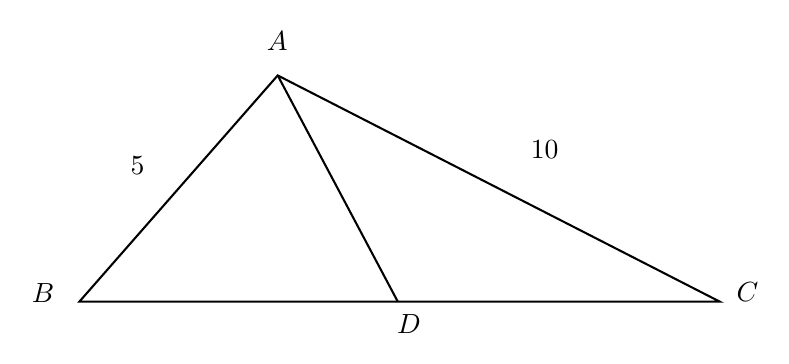
\begin{tikzpicture}[x=0.75pt,y=0.75pt,yscale=-1,xscale=1]
%uncomment if require: \path (0,300); %set diagram left start at 0, and has height of 300

%Shape: Triangle [id:dp9948603177891309] 
\draw   (206.76,70) -- (419.76,179) -- (111.2,179) -- cycle ;
%Straight Lines [id:da2482902118331296] 
\draw    (206.76,70) -- (264.59,178.92) ;

% Text Node
\draw (86.8,168.89) node [anchor=north west][inner sep=0.75pt]    {$B$};
% Text Node
\draw (200,47.49) node [anchor=north west][inner sep=0.75pt]    {$A$};
% Text Node
\draw (426.4,168.09) node [anchor=north west][inner sep=0.75pt]    {$C$};
% Text Node
\draw (134.4,107.53) node [anchor=north west][inner sep=0.75pt]    {$5$};
% Text Node
\draw (327.2,99.93) node [anchor=north west][inner sep=0.75pt]    {$10$};
% Text Node
\draw (262.8,183.73) node [anchor=north west][inner sep=0.75pt]    {$D$};


\end{tikzpicture}
\end{center}

By the cosine law, $\overline{BC} = 5\sqrt{7}$. Now we have the lengths of all sides of the triangle, we will invoke the \href{https://brilliant.org/wiki/stewarts-theorem/}{Stewart's theorem} but first we will find the lengths of $\overline{BD}$ and $\overline{DC}$ using the \textit{angle bisector theorem}, which states that 

\begin{equation}
    \dfrac{\overline{BD}}{\overline{AB}} = \dfrac{\overline{DC}}{\overline{AC}}
\end{equation}

\newpage

We will let $\overline{BD} = x$ and $\overline{DC} = 5\sqrt{7} - x$. By applying the \textit{angle bisector theorem}, we have:

\begin{equation*}
    \begin{array}{lll}
       \dfrac{\overline{BD}}{\overline{AB}} & = & \dfrac{\overline{DC}}{\overline{AC}}  \\
         
         \\
         
     \quad \dfrac{x}{5} & = & \dfrac{\sqrt{7} - x}{10} \\
     
        \\
         
     \quad 10x & = & 5\sqrt{7} - 5x    \\
     
      
         
     \quad x & = & \dfrac{\sqrt{7}}{3}     \\       
    \end{array}
\end{equation*}

Hence, $\overline{BD} = \dfrac{\sqrt{7}}{3} $ and $\overline{DC} = \dfrac{14\sqrt{7}}{3}$. Now we can now find the length of the angle bisector using Stewart's theorem:


\begin{center}



\tikzset{every picture/.style={line width=0.75pt}} %set default line width to 0.75pt        

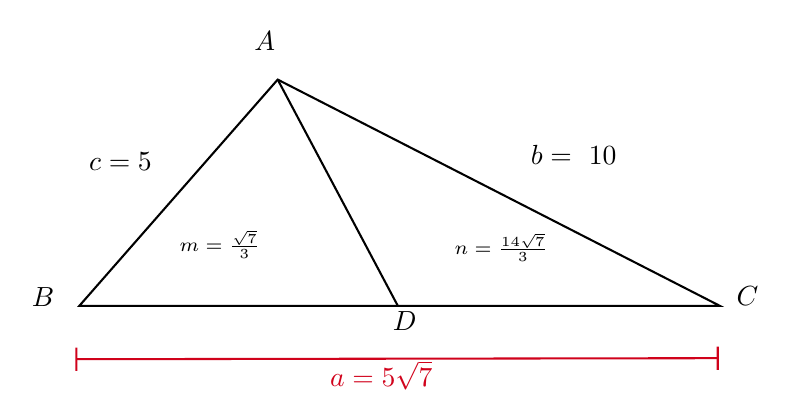
\begin{tikzpicture}[x=0.75pt,y=0.75pt,yscale=-1,xscale=1]
%uncomment if require: \path (0,447); %set diagram left start at 0, and has height of 447

%Shape: Triangle [id:dp26846802217349675] 
\draw   (196.76,221) -- (409.76,330) -- (101.2,330) -- cycle ;
%Straight Lines [id:da3901316108952435] 
\draw    (196.76,221) -- (254.59,329.92) ;
%Straight Lines [id:da9809013439693333] 
\draw [color={rgb, 255:red, 208; green, 2; blue, 27 }  ,draw opacity=1 ]   (99.78,355.72) -- (408.78,355.22) ;
\draw [shift={(408.78,355.22)}, rotate = 179.91] [color={rgb, 255:red, 208; green, 2; blue, 27 }  ,draw opacity=1 ][line width=0.75]    (0,5.59) -- (0,-5.59)   ;
\draw [shift={(99.78,355.72)}, rotate = 179.91] [color={rgb, 255:red, 208; green, 2; blue, 27 }  ,draw opacity=1 ][line width=0.75]    (0,5.59) -- (0,-5.59)   ;

% Text Node
\draw (76.8,319.89) node [anchor=north west][inner sep=0.75pt]    {$B$};
% Text Node
\draw (184,196.49) node [anchor=north west][inner sep=0.75pt]    {$A$};
% Text Node
\draw (416.4,319.09) node [anchor=north west][inner sep=0.75pt]    {$C$};
% Text Node
\draw (104.4,254.53) node [anchor=north west][inner sep=0.75pt]    {$c=5$};
% Text Node
\draw (317.2,250.93) node [anchor=north west][inner sep=0.75pt]    {$b=\ 10$};
% Text Node
\draw (250.8,331.23) node [anchor=north west][inner sep=0.75pt]    {$D$};
% Text Node
\draw (220.5,355.22) node [anchor=north west][inner sep=0.75pt]    {$\textcolor[rgb]{0.82,0.01,0.11}{a=5\sqrt{7}}$};
% Text Node
\draw (148,292.22) node [anchor=north west][inner sep=0.75pt]  [font=\scriptsize]  {$m=\frac{\sqrt{7}}{3}$};
% Text Node
\draw (280.5,293.72) node [anchor=north west][inner sep=0.75pt]  [font=\scriptsize]  {$n=\frac{14\sqrt{7}}{3}$};


\end{tikzpicture}
\end{center}

\vspace{-1em}

We will let the angle bisector be $d$, $AB = c, AC=b, BC = a, BD = m$ and $DC=n$. By theorem, we have:

\vspace{-1em}

\begin{equation*}
\begin{array}{lll}

   man + dad & =  &  bmb + cnc \\
    
    \\
   \left(\dfrac{\sqrt{7}}{3}\right)\left(5\sqrt{7}\right)\left(\dfrac{14\sqrt{7}}{3}\right) + (5\sqrt{7})(\overline{AD})^2 & = & (10)^2\left(\dfrac{\sqrt{7}}{3}\right)+ (5)^2\left(\dfrac{14\sqrt{7}}{3}\right)\\
     
     \\
     
    \left(\dfrac{\sqrt{7}}{3}\right)\left(\dfrac{14\sqrt{7}}{3}\right) + (\overline{AD})^2 & = & \left(\dfrac{20}{3}\right)+ \left(\dfrac{70}{3}\right)\\
       
       \\
       
 \quad \qquad \qquad \qquad \qquad \qquad \qquad \qquad  (\overline{AD})^2 & = & \dfrac{172}{9}\\
        
        \\
        
  \quad \quad \qquad \qquad \qquad \qquad \qquad \qquad \qquad  \overline{AD} & = & \dfrac{2\sqrt{43}}{3}
      
\end{array}
   
\end{equation*}

\vspace{-2em}

\newpage

Hence, the length of the angle bisector \fbox{$\overline{AD} = \dfrac{2\sqrt{43}}{3}$.}

\begin{probboxed}[IMO Shortlist, 2004]
Find all functions $f:\mathbb{R} \to \mathbb{R}$ satisfying the equation\[
	f(x^2+y^2+2f(xy)) = (f(x+y))^2.
\]for all $x,y \in \mathbb{R}$.
\end{probboxed}

\begin{rem}
I only determined one function. For those who are mathematicians reading this write-up, If you found other functions, then please, let me know. This is a perfect opportunity for me to learn more about functional equations. To do this, contact me at \mailto{jrdobaob@addu.edu.ph }.
\end{rem}

\ans{$f(x)=x$}

\sol

Based on our observations, it seems that the input in the left-handed side of the equation can be rewritten as a square of a binomial iff. $f(xy)=xy$ for some $a\in \mathbb{R}$. Because of this, we will make this as a claim that one of the functions that can be obtained out of this functional equation is $f(x)=x.$

\vspace{2mm}

\textit{Proof:}

\vspace{1mm}

Suppose $f(a)=a$ for $a\in \mathbb{R}$ is true. This implies that

\begin{equation*}
    \begin{array}{lll}
        f(x^2+y^2+2f(xy)) = (f(x+y))^2 & \implies & f(x^2 + y^2 + 2xy) = (x+y)^2 \\
        
        \\
        
        \qquad \quad f(x^2 + y^2 + 2xy) = (x+y)^2 & \implies & f\left((x+y)^2\right) = (x+y)^2 
    \end{array}
\end{equation*}

This proves our claim that $f(x) = x$ is true. Hence, we obtain a function.,
\begin{center}

\includegraphics[width=3.5in]{JOSH ROBERT OBAOB (2).png}
\end{center}



\end{document}
